\chapter{Modelling heat capacity} \label{chp:models}
    
    \textcolor{red}{Gabriel's comment: The original goal was to create a 0D model of the LTP thruster that could be compared to experiments. Prof. Higgins wanted an experimental line and a theory line on a graph that were somewhat on top of each other. Given that we received the V2 experiment parts to be setup at the end of April, I concentrated my efforts on getting the thruster running so we could get experimental data. Due to reasons explored in the discussion chapter, more parts had to be made for the V2 experiment to work. I ended up without experimental data and without this model completed. This is the reason Prof. Higgins dismissed my thesis in August, and I attempted a re-scoping of the work toward designing and commissioning the V2 thruster. I will have to change the justification of why this chapter was written if I keep it.}

    To correctly predict the temperature increase of the gas that should be expected when laser energy is input, the heat capacity of argon and hydrogen was modelled. Argon is the current gas used in experiments, as it is economical and easy to ionize. Hydrogen is projected to be used in the full-scale LTP engine for its increased $I_\mathrm{sp}$ due to having lower molecular weight.

    \section{Equilibrium calculations} \label{sec:equilibrium calcs}
        
        The following seventh order polynomials and their coefficients ($a_1$ to $a_7$, $b_1$, and $b_2$), from \textcite{mcbrideNASAGlennCoefficients2002}, were implemented in Python. Species of interest were \ce{H}, \ce{H2}, \ce{Ar}, \ce{Ar+}, and electrons \ce{e-}. Plasma temperatures studied allowed us to treat the argon as singly ionized, and the hydrogen as dissociated. The heat capacity at constant pressure, as well as the temperature ($T$) dependent part of enthalpy and entropy of each species are given by $C_p^0$, $H^0$ and $S^0$, respectively. $\bar R$ is the universal gas constant.

        \begin{equation}
            C_p^0 (T)/\bar R = a_1 T^{-2} + a_2 T^{-1} + a_3 + a_4   T + a_5 T^2 + a_6 T^3 + a_7 T^4
        \end{equation} 
        
        \begin{equation}
            H^0 (T)/\bar RT = -a_1 T^{-2} + a_2 \ln(T)/T + a_3 + a_4 T / 2 + a_5 {T^2}/3 + a_6 {T^3}/4 + a_7 {T^4}/5 + b_1/T
        \end{equation}
        
        \begin{equation}
            S^0(T)/\bar R = -a_1 T^{-2}/2 - a_2 T^{-1} + a_3\ln(T) + a_4   T + a_5 {T^2}/2 + a_6 T^3/3 + a_7 T^4/4 + b_2
        \end{equation}

        Next, the functions for entropy $\bar s_i$ of each species $i$ and Gibbs energy $\bar g_i$, both per \unit{kmol}, were implemented. These values depend on temperature $T$ and partial pressure $p_i$. $y_i$ is the molar fraction of the species, and $p_{ref}$ is the reference pressure, equal to \qty{1}{bar}.
        
        \begin{equation}
            \bar s_i (T, p_i) = \bar s_i^0 (T) - \bar R \ln \frac{y_i p}{p_{ref}}
        \end{equation}

        \begin{equation}
            \bar g_i = \bar h_i - T \bar s_i
        \end{equation}

        Considering the number of moles $n_i$, expressions of the Gibbs energy of the two mixtures $G_{mixture}$ are found:

        Starting with \qty{1}{kmol} argon,
        \begin{equation}
            G_{mixture,\: Ar}(T, p) = n_{Ar} \bar g_{Ar}(T, p_{Ar}) + n_{Ar+} \bar g_{Ar+}(T, p_{Ar+}) + n_e \bar g_e(T, p_e)
        \end{equation}

        Starting with \qty{1}{kmol} hydrogen,
        \begin{equation}
            G_{mixture,\: H_2}(T, p) = n_H \bar g_H(T, p_H) + n_{H2} \bar g_{H2}(T, p_{H2})
        \end{equation}

        \autoref{fig:Gibbs} plots the Gibbs energy of the hydrogen mixture as a function of its degree of dissociation $x$, for different total pressures $p$.

        \begin{figure}[!ht]
            \centering
            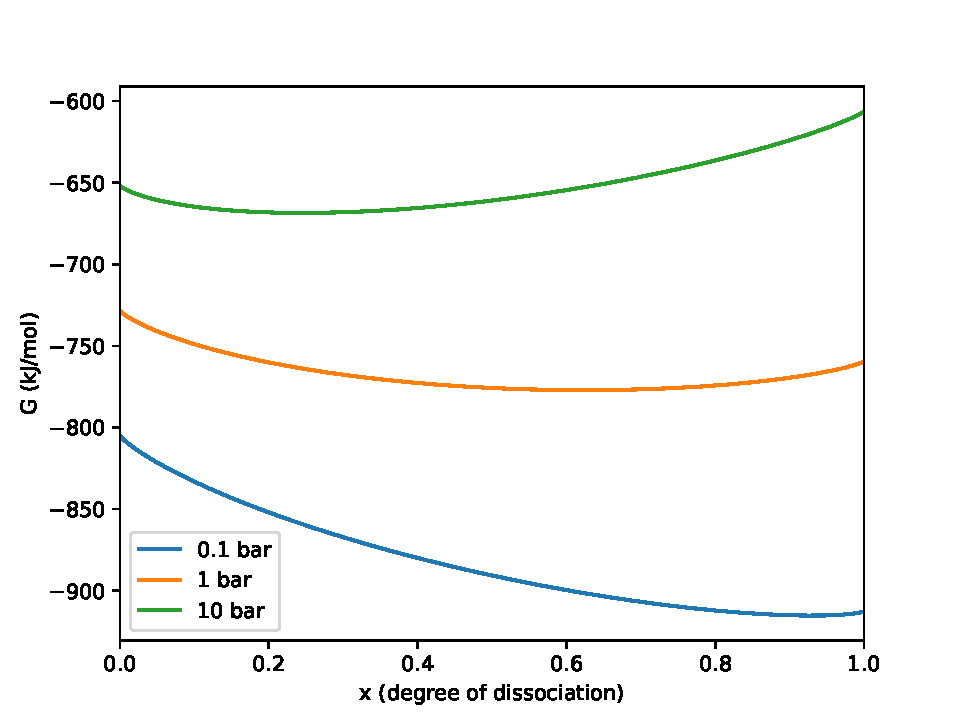
\includegraphics[width=0.7\textwidth]{assets/2 models/Gibbs.pdf}
            \caption{Gibbs free energy (G) plotted against the degree of dissociation (x) of hydrogen under three different pressures}
            \label{fig:Gibbs}
        \end{figure}

        A similar dissociation graph can be found with argon, but with three species. The Gibbs energy is then minimized to determine the molar fractions $y_i$ at which the mixture reaches equilibrium. From this, the enthalpy $H$ of the mixture was found. The $C_p$ of the mixture was then calculated from the enthalpy with:

        \begin{equation}
            C_p = \frac{\partial H}{\partial T}
        \end{equation}
        
        For argon, these calculated $C_p$ values were validated against values from CEA \cite{CEARUNRev4} in \autoref{fig:Cp_compare}.
        
        \begin{figure}[!ht]
            \centering
            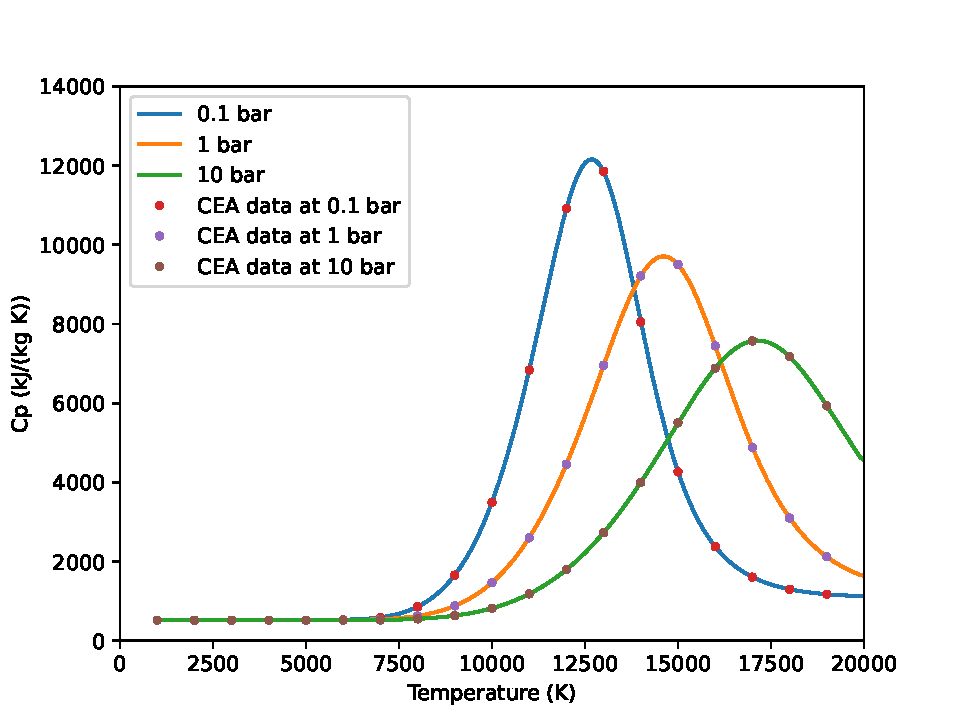
\includegraphics[width=0.7\textwidth]{assets/2 models/Cp_compare.pdf}
            \caption{Comparing calculated $C_p$ values of argon to those from CEA}
            \label{fig:Cp_compare}
        \end{figure}

    % \section{Test problem for heat addition}

    %     With these variable heat capacities, a test problem can be solved, giving a preliminary 0D model of an LTP engine.

    %     Bla bli \todo{Add homework problem}